\documentclass[twocolumn]{article} 
%use IEEE Computer Science Society style 
\usepackage{styles/latex8}
%Setting the graphicspath
\usepackage{graphicx}
\graphicspath{{images/}} 

%print institute affiliation
\usepackage[affil-it]{authblk}
%draw figures
\usepackage{tikz}
%draw gantt charts
\usepackage{styles/gantt}
%draw horizontal  rules in tables
\usepackage{booktabs}
%enable multipage table header repeat
\usepackage{xtab}
%enable set width columns in xtabular
\usepackage{array}
%enable caption in xtabular tables
\usepackage{caption}
%enable \Verb command inside tables
\usepackage{fvextra}
%enable math equations
\usepackage{amsmath}
%drawing algorithms
\usepackage{algorithm}
\usepackage{algorithmic}

%output code listings : 3 packages
\usepackage{listings}
%\usepackage[T1]{fontenc}
%\usepackage{lmodern}

%creates a box named \codebox to store code listings
\newsavebox{\codebox}% For storing  code listings
%create \defcolor command to point to color of gantt bar
\newcommand{\defcolor}{red}
%create \flow command to point to rightleftharpoons character
\newcommand{\flow}{\rightleftharpoons}

\begin{document}
\title{Template  LaTeX Document}
\author{Valerii Klymchuk}
\affil{Department of Mathematics, University of California, Berkeley}
%\institute{Centre for Modern Templates}
\maketitle

\begin{abstract}
Smartphones are increasingly being used to store personal information as well as to access sensitive data from the Internet and the cloud. Establishment of the identity of a user requesting information from smartphones is a prerequisite for  secure systems in such scenarios. In the past, keystroke-based user identifiation has been successfully deployed on production-level mobile devices to mitigate the risks associated with naive username/password based authentication. However, these approaches have two major limitations: they are not applicable to services where authentication occurs outside the domain of the mobile
device such as web-based services; and they often overly tax the limited computational capabilities of mobile devices.

In this paper, we propose a protocol for keystroke dynamics analysis which allows web-based applications to make use of remote attestation and delegated keystroke analysis. The end result is an efficient keystroke-based user identification mechanism that strengthens traditional password protected services
while mitigating the risks of user profiling by collaborating malicious web
services. We present a prototype implementation of our protocol using
the popular Android operating system for smartphones.
\end{abstract}

\section{Introduction} 
This is going to be a normal paragraph in our introduction. 


\subsection{Some Background} 
Some more stuff. 

\subsubsection{Drilled Down}\label{sec:drilled-down}
More information here. 

\section{Tables, figures and subfiles}\label{sec:background}

\subsection{Tables and Figures}

To insert a figure, you can use the TeXnicecenter menus. 
\begin{figure}
	\centering
		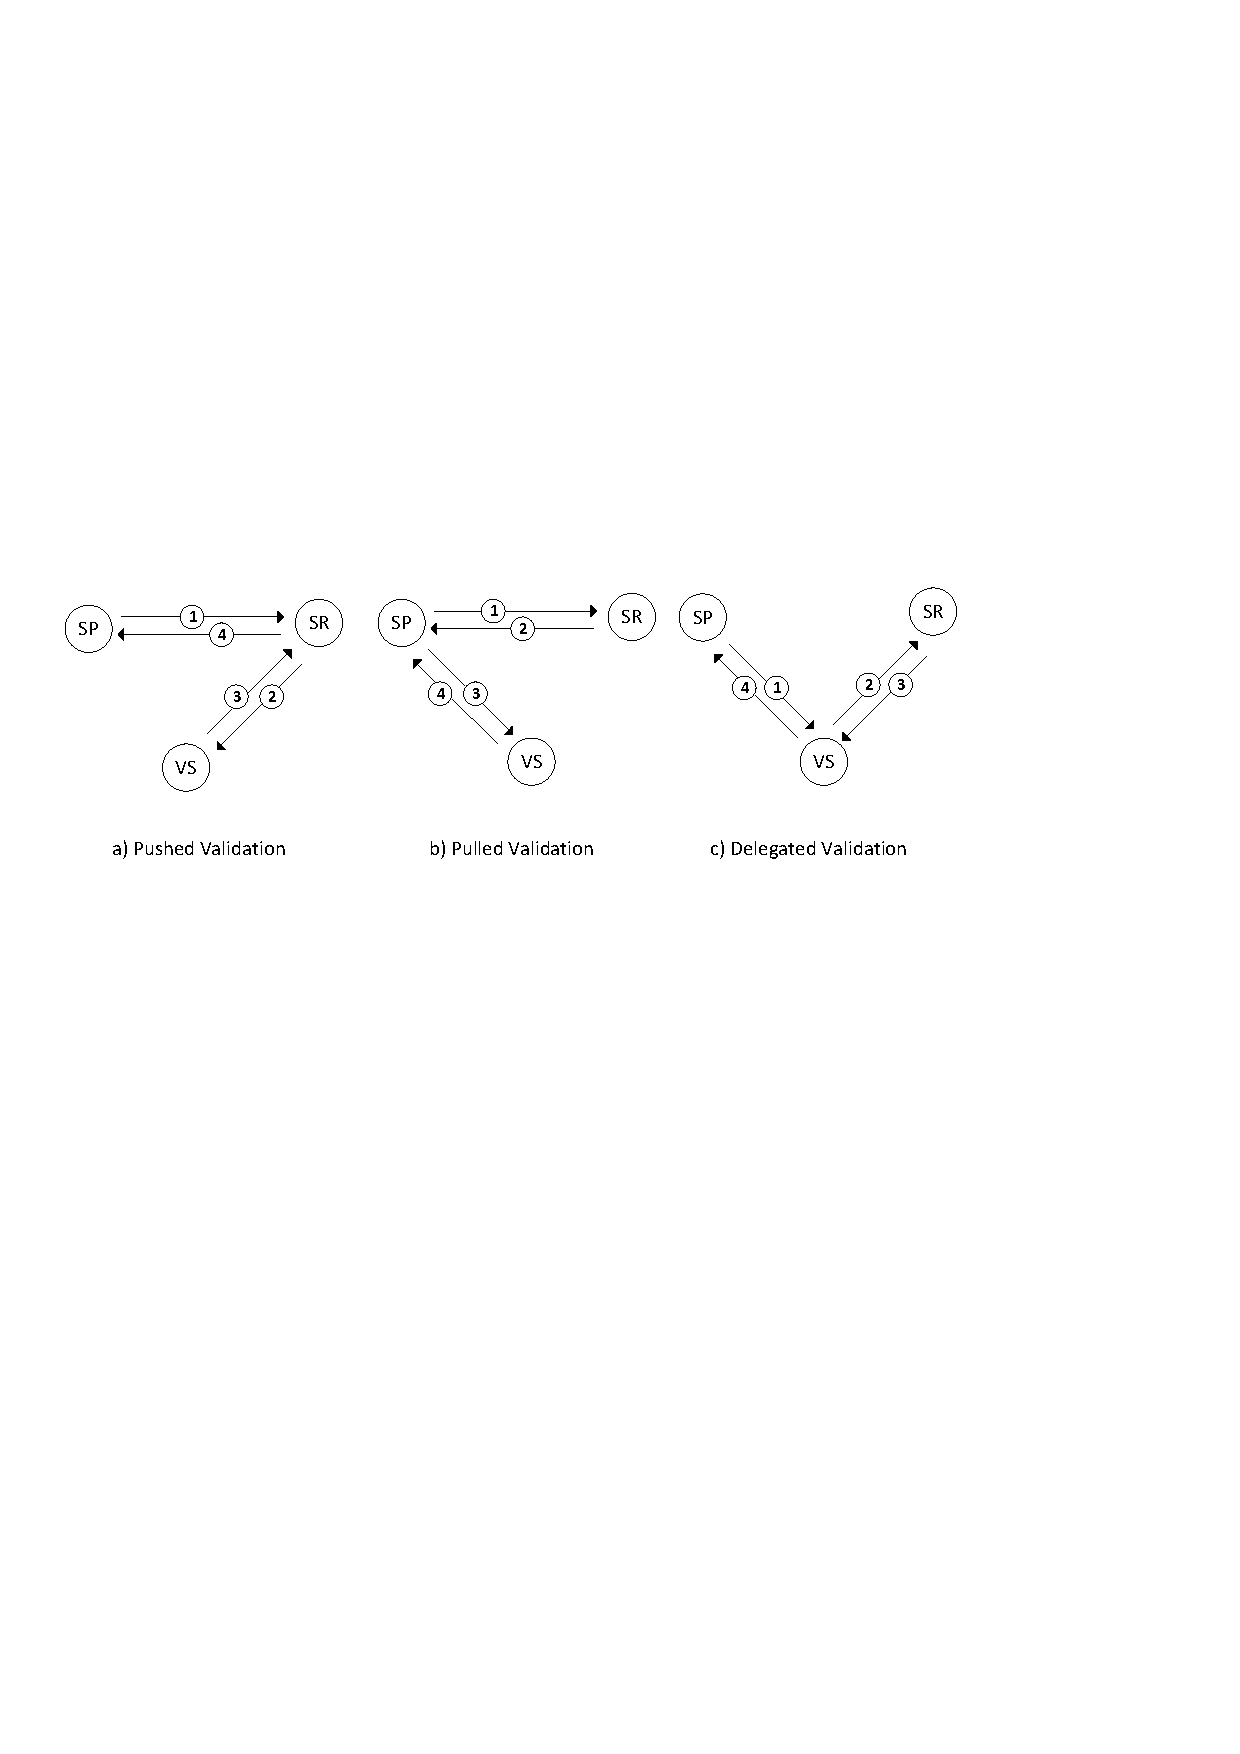
\includegraphics[width=\linewidth]{att-models-base.pdf}
	\caption{My First Figure}
	\label{fig:att-models-base}
\end{figure}



\begin{figure}
	\centering
	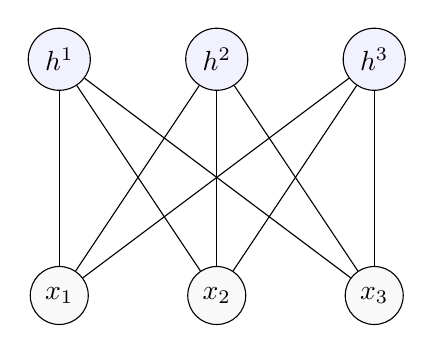
\begin{tikzpicture}	
	\tikzset{
		hcirc/.style={
			draw, circle, fill=blue!5
		},
		xcirc/.style={
			hcirc, fill=gray!5
		}
	}
	
	\foreach \i in {1, ..., 3}{
		\node [hcirc] (h\i) at (\i*2,3) {$h^\i$};
	}
	
	\foreach \i in {1, ..., 3}{
		\node [xcirc] (x\i) at (\i*2,0) {$x_\i$};
	}
	
	\foreach \i in {1, ..., 3}{
		\foreach \v in {1, ..., 3}{
			\path (h\i) edge [draw] (x\v);
		}
	}
	\end{tikzpicture}	
	\caption{Drawn tikzpicture} \label{fig:M1}
\end{figure}

Now for a table! 

\medskip
%\begin{table}
\tablefirsthead{
\toprule  & \bf document class  &\bf bibliography style &   \\ \midrule}
\tablehead{
\multicolumn{4}{c}{\text{\tablename~\thetable{}  continued }} \\
\midrule &\bf document class &\bf bibliography style &  \\ \midrule}
\tablecaption{Document and bibliograpghy styles}
\label{tab:MyFirstTable}
\begin{xtabular}{
		%@{}	
		p{0.21\linewidth}
		p{0.26\linewidth}
		p{0.21\linewidth}
		p{0.11\linewidth}
	    %@{}
    }
	Institute of Electrical and Electronics Engineers &\Verb|IEEEtran| & \Verb|IEEEtran|& \raisebox{-0.5\totalheight}{
\includegraphics[width=1\linewidth]{ieee.png}}\\ 
	\midrule
	Association for Computing Machinery & \Verb|sig-alternate|  & \Verb|plain| & \raisebox{-0.5\totalheight}{
\includegraphics[width=1\linewidth]{acm.jpeg}}   \\ 
	\midrule
	Lecture Notes in Computer Science& \Verb|llncs|& \Verb|llncs|& \raisebox{-0.5\totalheight}{
\includegraphics[width=1\linewidth]{llncs.png}} \\ 
	\midrule
	IEEE Computer Society                             & {\Verb|[twocolumn]| \verb|{article}|  \Verb|\usepackage|  \Verb|{latex8}|} & \Verb|IEEEtran|                & \raisebox{-0.5\totalheight}{
\includegraphics[width=1\linewidth]{ieeecs.jpg}} \\ 
	\midrule
	General & \Verb|article|  & \Verb|plain|  &  \\ 
	\bottomrule
\end{xtabular}
%\end{table}
%\caption{Sample multipage table with repeating header}
%\label{tab:MyFirstTable}


\subsection{Cross-references} 
Some text here that wants to refer to Table~\ref{tab:MyFirstTable}. You can also refer to the Figure~\ref{fig:att-models-base}. When you want to refer to a previous section, you can use the \verb|\ref| command again. Section~\ref{sec:background} and Section~\ref{sec:drilled-down}. 

\subsection{Sub section through input command}
This comes from a separate file. Notice that we have this subsection included in the Navigator.  


\section{Displaying Mathematics}

\LaTeX\ is extremely powerful when it comes to typesetting mathematics. It's one of the core strengths of this system. 

There are two ways of displaying maths. One is \emph{inline} and the other is \emph{display} format -- in which the whole math sits on its own set of lines.


\subsection{Inline Mode}
We are going to insert a mathematics equation inline here using a pair of \$ signs: $E=mc^2$   . As you can see, the display (such as line spacing) does not get messed up by the mathematics as it does with word processing softwares. 

\subsection{Display Mode}
We can also display equations in their own set of lines. To do this, we can use the equation environment. 

\begin{equation}\label{eq:emc}
E=mc^2
\end{equation}

As you can see, \LaTeX\ inserts the equation number automatically. We can refer to it using the \verb|\ref| command just as we referred to sections, figures and tables. (E.g. Equation~\ref{eq:emc}.) To get rid of the equation number, simply use the \emph{star variant} of the equation environment. (For this, you need the \texttt{amsmath} package.)

\begin{equation*}
E=mc^2
\end{equation*}

Alternatively, we can use the shorthand keys \verb|\[| and \verb|\]|
\[
E=mc^2
\]


\section{Mathematical Features}
\LaTeX\ has many builtin features and you can get many more easily. Here, we'll see some of these features: 

Addition, subtraction, multiplication and division: 

\[
x+2 - 25 \times 35 \div 98 
\]

Superscripts and subscripts: 

\[ x^2  \]
\[ x_{(i)} \]


Summation, union, intersection, big-union, integral: 

\[ \sum_{i=1}^{n}{i^2} \]
\[ x \cup y \cap z \]
\[ \bigcup_{i=1}^{n}{x_i} \]
\[ \int_0^n{x^2} \]

Fractions, brackets, square root: 

\[ \frac{x}{y} \]
\[ \frac{\sum_i{x^2}}{\int_0^n{x^2}} \]
\[ \sqrt{\frac{\sqrt{36}} {x^5}} \]

\[ 2 \times \left( \frac{34}{\frac{124}{356}}    \right)  \]

Greek letters: 

\[
\alpha + \beta + \gamma^* + \Sigma + \Theta + 2_\epsilon 
\]

Matrices and vectors. For this, you need to include the \texttt{amsmath} package and then use the \texttt{bmatrix} or \texttt{pmatrix} environment: 

\[
\begin{pmatrix}
\frac{a}{44} & b \\ 
c & \sqrt{d} 	
\end{pmatrix}
\]

Accents: 

\[ \hat{x} \]
\[ \hat{\imath} \] 
\[ \dot{x} \]

See the \texttt{Math} menu in the IDE for other operations. You can refer to ``Short Math Guide for \LaTeX'' for a lot more examples. 

\section{Using Symbols}
You might come across situations where you need to find new symbols. For this, you can refer to the ``The Comprehensive \LaTeX Symbols List''.  

\[ x \rightleftharpoons  y \]



(Optional) Since this is a long command, we might want to create a shortcut using the \verb|\newcommand| command in the preamble. This also allows us to later change the symbol without having to change the equations. 

\[ x \flow y \]



\section{Gantt chart}

\begin{figure*}
	\centering
	\resizebox{\linewidth}{!}{
		\begin{gantt}[drawledgerline=true]{11}{24}
			% vertical, horizontal 'boxes'
			\begin{ganttitle}
				\numtitle{2012}{3}{2012}{10}
				% start, label, width 
				\numtitle{2013}{1}{2013}{12}
				\numtitle{2014}{1}{2014}{2}
			\end{ganttitle}
			\begin{ganttitle}
				\numtitle{3}{1}{12}{1}
				% start, skip, end, width 
				\numtitle{1}{1}{12}{1}
				\numtitle{1}{1}{2}{1}
			\end{ganttitle}
			\ganttmilestone{Proposal Defense}{0} % Label, position
			%=======================================
			\ganttgroup{Background Study}{0}{6} % start, width 
			\ganttbar[color=\defcolor]{Android Security}{0}{3}
			\ganttbarcon[color=\defcolor]{Code Analysis}{3}{2}
			\ganttbarcon[color=\defcolor]{Policy Mechanisms}{5}{1}
			\ganttmilestonecon{Literature Review Complete}{6}
			% notice the 'con' at the end -- for continue 
			%=======================================
			\ganttbarcon[color=\defcolor]{
				\textbf{Formal Specification} % can format labels!
			}{6}{6}
			\ganttmilestonecon{Spec Document}{12}
			%=======================================
			\ganttbar[color=blue]{Thesis and Paper Writing}{0}{24}
		\end{gantt}
	}
	\caption{Gantt Chart} \label{fig:G1}
\end{figure*}

\section{Algorithms}

\begin{algorithm}
	\begin{algorithmic}[2]
		\REQUIRE{Randomly populated array}
		\ENSURE{Sorted array}
		\IF{$i\leq0$}
		\STATE $i\gets1$
		\ELSE 
		\IF{$i\geq0$} \label{line:impline}
		\FOR{$j=0$ \TO $10$}
		\STATE blah()
		\STATE carryOutSomeProcessing() \label{line:mostimp}
		\ENDFOR
		\ENDIF
		\ENDIF
		\RETURN i
	\end{algorithmic}
	\caption{My First Simple Algorithm}
	\label{algo:first}
\end{algorithm}

And of course, we can refer to the algorithm using \verb|\ref|: See Algorithm~\ref{algo:first} but the good thing is we can also refer to a specific line e.g. Line~\ref{line:impline} or Line~\ref{line:mostimp}.


\section{Code listings}

\lstset{language=c++, float=H}
\lstset{caption=Some C++ Code}
%\begin{adjustbox}{width=0.418\textwidth}
\begin{lstlisting}[frame=single, label=lst:lowertri]{}
for(i = 0; i < 10; i++){
// increment the pointer
*p++ = i;
}
\end{lstlisting}

%\end{adjustbox}


%output code from text file
%\lstset{language=java,frame=single,basicstyle=\ttfamily,numbers=left}
%\lstinputlisting[caption=Signing,label=lst:lowertri]{Sign.java}


And we can refer to Listing~\ref{lst:lowertri} in text.



\section{Bibliography styles} 

The following table contains specifications for document style and bibliography style as requested by major publications.

%\begin{table}
\tablefirsthead{
	\toprule  & \bf document class  &\bf bibliography style &   \\ \midrule}
\tablehead{
	\multicolumn{4}{c}{\text{\tablename~\thetable{}  continued }} \\
	\midrule &\bf document class &\bf bibliography style &  \\ \midrule}
\tablecaption{Document and bibliograpghy styles}
\label{tab:MyFirstTable1}
\begin{xtabular}{
		p{0.20\linewidth}
		p{0.26\linewidth}
		p{0.19\linewidth}
		m{0.11\linewidth}
	}
	Institute of Electrical and Electronics Engineers &\Verb|IEEEtran| & \Verb|IEEEtran|& \raisebox{-0.5\totalheight}{
\includegraphics[width=1\linewidth]{ieee.png}}\\ 
	\midrule
	Association for Computing Machinery & \Verb|sig-alternate|  & \Verb|plain| & \raisebox{-0.5\totalheight}{
\includegraphics[width=1\linewidth]{acm.jpeg}}   \\ 
	\midrule
	Lecture Notes in Computer Science& \Verb|llncs|& \Verb|llncs|& \raisebox{-0.5\totalheight}{
\includegraphics[width=1\linewidth]{llncs.png}} \\ 
	\midrule
	IEEE Computer Society                             & {\Verb|[twocolumn]| \verb|{article}|  \Verb|\usepackage|  \Verb|{latex8}|} & \Verb|IEEEtran|                & \raisebox{-0.5\totalheight}{
\includegraphics[width=1\linewidth]{ieeecs.jpg}} \\ 
	\midrule
	General & \Verb|article|  & \Verb|plain|  &  \\ 
	\bottomrule
\end{xtabular}
%\caption{Document and bibliograpghy styles with repeating header}
%\label{tab:MyFirstTable1}
%\end{table}

\medskip
Using and managing bibliographies in \LaTeX\ is very easy. 
These are the steps required to use them: 

\begin{enumerate}
	\item Create a main document file 
	\item Collect bibliography entries in a \verb|.bib| file. For this: 
	\begin{itemize}
		\item Get the bibliography from Google Scholar/ACM or where ever or 
		\item Write the entry yourself. 
	\end{itemize}
	\item Add a \verb|\bibliographystyle| and a \verb|\bibliography| command to your document. 
	\item \emph{Cite} the references where you need using the key. 
	\item Build the file a couple of times to get the citations in the main document. 
\end{enumerate}




\section{Bibliography citations}
We are going to use this section to put some text in our document and at some points, we are going to inset a reference table~\ref{tab:MyFirstTable1}. This, for example, is going to turn into a reference~\cite{lecun2015deep}. This ~\cite{webster1984specific} is yet another reference. And so on.~\cite{nauman2010apex}

This is going to be a new paragraph.



% -------------------------------------------------------------------
% add bibliography-related commands here 


\bibliography{bibfile}
\bibliographystyle{IEEEtran}

\end{document} 